\section[Jaderná bezpečnost \& ochrana do hloubky]{Základní principy jaderné bezpečnosti a ochrana do hloubky}

\subsection{Princip 3S}

3S = Safety, Security, Safe Guards

Pro zajištění mírového a bezpečného využívání jaderné energie a prevenci zneužití jaderných materiálů je nezbytné vytvořit legislativní a regulační rámec. V této souvislosi se v oblasti jaderného průmyslu používají a aplikují tři sféry (pojmy), jež vyjadřují různé formy bezpečnosti:

\begin{itemize}
    \item \textbf{Bezpečnost/Safety} = Dodržovat provozní podmínky, předcházet nehodám a zmírňovat následky nehod. Vše s ohledem na ochranu pracovníků, veřejnosti a životního prostředí.

    V praxi to znamená, že zajistit bezpečný provoz znamená prokázat, že jaderné zařízení neohrožuje svým fungováním bezprostřední okolí ani zaměstnance a uživatele reaktoru.

    \underline{Příklad u nás na reaktoru VR1:} Bezpečnost jaderného zařízení je prokazována v oblasti jaderné bezpečnosti, radiační ochrany a havarijní připravenosti. Na pracovišti je vymezeno kontrolované pásmo, ve kterém je zabezpečeno nepřetržité monitorování prostředí i osob. Vstup do kontrolovaného pásma je povolen pouze poučeným osobám splňujícím podmínky vstupu. Prostor haly je monitorován systémem RMS (Radiační monitorovací systém), který je doplněn termoluminiscenčními detektory a potřebným množstvím přenosných přístrojů. Obsluha reaktoru je monitorována pomocí filmového a elektronického dozimetru, ostatní osoby vstupující do kontrolovaného pásma jsou vybaveny elektronickými dozimetry. Roční hodnota efektivní dávky od gama záření je pro pracovníky zpravidla menší než 0,5 mSv (povolená roční efektivní dávka pro radiační pracovníky je stanovena na 20 mSv za rok), u návštěvníků a studentů se pohybuje pod prahem citlivosti měřicích přístrojů

    \begin{itemize}
        \item \textbf{Jaderná bezpečnost} = Stav a schopnost jaderného zařízení a fyzických osob obsluhujícíh jaderné zařízení, aby byla zajištěna kontrola štěpné řetězové reakce, odvod tepla z AZ, zabránění úniku RA látek či IZ do ŽP a omezit následky nehod.

        Schopnost zařízení vychází z projektu a konstrukce zařízení, lze zvyšovat pravidelnou inovací a modernizací zařízení. Stav zařízení vystihuje aktuální stav zařízení. Zařízení je v dobrém stavu udržováno díky náležité údržbě a provozním kontrolám (např. kontrola reaktorových nádob a vnitřních částí, stav a provozuschopnost absorpčních tyčí nebo testy systému ochran řízení). Schopnost obsluhy hodnocena již při výběru vhodných pracovníků, kdy jsou hodnoceny odborné znalosti, ale také osobnostní charakteristiky. Schopnost obsluhy vychází z kvalitní odborné přípravy a je ověřována zkušební komisí SÚJB. Schopnost obsluhy je zvyšována (a ověřována) v rámci další odborné přípravy a periodického školení. Stav obsluhy dána aktuálním fyzickým stavem a psychickým rozpoložením. Díky pravidelnému ověřování osobnostní a zdravotní způsobilosti jsou vytvářeny podmínky, aby stav obsluhy odpovídal vysokým nárokům.

        \item \textbf{Radiační ochrana} = Ochrana pracovníků, veřejnosti a životního prostředí před rizikem ionizujícího záření pomocí technických a organizačních opatření.
        
        \item \textbf{Připravenost k odezvě na RMU} = Spojeno s rozpoznáním a reakcí na mimořádnou událost, která může při provozu vniknout.
        
        RMU = událost, která vede nebo může vést k překročení limitů ozáření a která vyžaduje opatření, jež by zabránila jejich překročení nebo zhoršování situace z pohledu zajištění radiační ochrany.

        \item \textbf{Radiační mimořádná událost prvního stupně} = RMU zvládnutelná silami a prostředky obsluhy nebo pracovníků vykonávajících práci v aktuální směně osoby, při jejíž činnosti radiační mimořádná událost vznikla.
        
        \item \textbf{Radiační nehoda} = RMU nezvládnutelná silami a prostředky obsluhy nebo pracovníků vykonávajících práci v aktuální směně osoby, při jejíž činnosti radiační mimořádná událost vznikla, nebo vzniklá v důsledku nálezu, zneužití nebo ztráty radionuklidového zdroje, která nevyžaduje zavedení neodkladných ochranných opatření pro obyvatelstvo.
        
        \item \textbf{Radiační havárie} = RMU nezvládnutelná silami a prostředky obsluhy nebo pracovníků vykonávajících práci v aktuální směně osoby, při jejíž činnosti radiační mimořádná událost vznikla, nebo vzniklá v důsledku nálezu, zneužití nebo ztráty radionuklidového zdroje, která vyžaduje zavedení neodkladných ochranných opatření pro obyvatelstvo.
        
    \end{itemize}

    \item \textbf{Zabezpeční/Security} = Prevence, detekce a včasná odezva na krádež, sabotáž, neautorizované vstupy, nelegální převoz a další akce zahrnující jaderné a radioaktivní materiály.
    
    Neboli: zabezpečení pracoviště je takové aby zabránilo k záměrnému zneužití či poškození zařízení a nebo k neoprávněným manipulacím s jaderným materiálem.

    \underline{Příklad u nás na reaktoru VR1:} Zabezpečení pracoviště vychází ze základních funkcí fyzické ochrany, jako je včasná detekce útočníka, jeho zpomalení a adekvátní zásah. Fyzická ochrana reaktoru a jaderných materiálů, které se na něm používají, splňuje požadavky vyhlášky SÚJB o zabezpečení jaderných materiálů a jaderných zařízení, která vychází z doporučení Mezinárodní agentury pro atomovou energii.

    \begin{itemize}
        \item \textbf{Fyzická ochrana} = Systém technických a organizačních opatření zabraňující neoprávněným činnostem s jaderným zařízením nebo jaderným materiálem.
        \item \textbf{Kybernetická bezpečnost} = Zajištění bezpečnosti kybernetického prostoru -- HW, SW, počítačové sítě, ...\item \textbf{Ochrana informací} = Ochrana a nakládání s citlivými informacemi, jsou to informace ovlivňující bezpečnost (omezené, důvěrné, tajné), souvisí s kybernetickou bezpečností a fyzickou ochranou.
    \end{itemize}
    
    \item \textbf{Zárukový proces/Safeguards} = Včasnou detekcí zneužití jaderných materiálů nebo technologií zabránit šíření jaderných zbraní, poskytnutí záruky, že státy využívají jaderný materiál a jaderná zařízení pouze pro mírové účely.

    Znamená: Reaktor, resp. jaderné zařízení musí být provozováno dle pravidel stanovených smlouvou o nešíření jaderných zbraní. Zárukový proces zajišťuje permanentní evidenci a kontrolu všech jaderných materiálů na pracovišti reaktoru.

    \underline{Příklad u nás na reaktoru VR1:} Základním kamenem zárukového procesu na pracovišti reaktoru je systém evidence a kontroly všech držených štěpných jaderných materiálů. Každá položka jaderného materiálu je sledována, má přesně definované místo svého uložení a svůj inventární záznam. Přesuny a manipulace jaderných materiálů lze provést pouze se souhlasem vedoucího evidence jaderných materiálů a tyto změny musí být zavedeny do evidenčních záznamů.

    Mezinárodní dohody členských států IAEA:

    \begin{itemize}
        \item \textbf{Treaty on the Non-Proliferation of Nuclear Weapon} = Dohoda o nešíření jaderných zbraní
        \item Dohoda o zárukách
        \item Výměna informací = Hlášení informací spojených se zárukovým procesem národním koordinátorům a IAEA.
    \end{itemize}

    \textbf{Forenzika} = Nástroje a metody pro vyšetřování zneužití jaderných materiálů, neschválené aktivity.

\end{itemize}

Může být těžké rozlišit bezpečnost a zabezpečení. \textbf{Zabezpečení} je spojeno se zlým úmyslem, cílenou akcí lidí, která může ohrozit další lidi, hrozba směřuje z okolí směrem do zařízení. \textbf{Bezpečnost} zahrnuje širší otázky ohrožení lidí (nebo životního prostředí) radiací, bez ohledu na primární příčinu, hrozba směřuje od zřízení směrem do okolí.

\subsection{Principy bezpečného využívání jaderné energie}

V rámci bezpečnosti jaderného zařízení, jehož součástí je jaderný reaktor je provozovatel (držitel lincence) nucen, aby bylo za každé situace zajištěno plnění základních bezpečnostních funkcí, přičemž v analýzách prokazování uvažuje jednoduchou poruchu a hermetičnost kontejmentu.

\subsubsection{Bezpečnostní funkce}

Splnění všech bezpečnostních funkcí je nezbytné pro zajištění jaderné bezpečnosti.

\begin{itemize}
    \item \textbf{Kritická bezpečnostní funkce} = ochrana celistvosti jedné nebo více fyzických bariér proti úniku RA látek.
    \item Musí být zachovány i při selhání nebo nesprávné činnosti jednotlivých zařízení a chybě obsluhy $\rightarrow$ musí být zahrnuto v projektu.
    \item Splnění základních bezpečnostních funkcí musí být zajištěno ve všech provozních stavech a ve všech etapách
    životního cyklu JZ.
\end{itemize}

Základní bezpečnostní funkce podle §45 odst. 2 AtZ, a §2 písm. b) vyhl. 329/2017 Sb.:

\begin{itemize}
        \item umožňovat v případě potřeby okamžitě a bezpečně odstavit jaderný reaktor a udržovat jej v podkritickém stavu
        \item zabránit nekontrolovanému rozvoji štěpné řetězové reakce
        \item fyzikálně znemožnit vznik kritického a nadkritického stavu mimo vnitřní prostor jaderného reaktoru
        \item zajišťovat odvod tepla vytvářeného jaderným palivem a technologickými systémy
        \item zajistit stínění a zabránit úniku radioaktivní látky a šíření ionizujícího záření do životního prostředí
    \end{itemize}

Základní bezpečnostní principy:

\begin{itemize}    
	\item \textbf{Administrativní opatření} = opatření pro řízení a ověřování bezpečnosti
 
	\item \textbf{Technická opatření} = technické principy uplatněné v celém životním cyklu zařízení
        \begin{itemize}
            \item \textbf{Diverzita} = různorodost, různé principy, technologie, výrobci $\rightarrow$ snaha o vyloučení poruchy ze společné příčiny
             \item \textbf{Redundance} = zálohování, vícenásobné použití $\rightarrow$ omezení jednoduché poruchy, eliminace stochastických poruch
            \item \textbf{Nezávislost} = využití rozdílných metod, zdrojů
            \item \textbf{Separace} = fyzické oddělení systémů $\rightarrow$ ochrana proti externím vlivům (společná příčina)
        \end{itemize}
 
    \item \textbf{Kultura bezpečnosti} = Soubor charakteristik a postojů organizace i jednotlivců zajišťující, že otázkám ochrany a bezpečnosti je věnována priorita odpovídající jejich významu. Individuální i kolektivní závazek k bezpečnosti ze strany personálu na všech úrovních (včetně vedení a středního managementu). Odpovědnost organizace i jednotlivců za dodržování pravidel bezpečnosti. Podpora vzdělávání a budování prostředí otevřeného dotazům spojeným s plněním bezpečnosti. Chování managementu funguje jako vzor v pozitivním i negativním smyslu.

    Principy kultury bezpečnosti:

    \begin{itemize}
        \item Individuální i kolektivní závazek k bezpečnosti ze strany personálu na všech úrovních (včetně vedení a středního managementu).
        \item Osobní odpovědnost za bezpečnost.
        \item Vedoucí pracovníci demonstrují svoje postoje k bezpečnosti.
        \item Respekt vůči jaderné technologii.
        \item Při rozhodování platí "bezpečnost na prvním místě".
        \item Trvalé ověřování úrovně bezpečnosti..
        \item Poučení se z chyb
    \end{itemize}
\end{itemize}

\subsubsection{Přístup třístupňové ochrany}

\begin{itemize}
    \item \textbf{Prevence} = Základ všeho. Předchází vzniku problémů a snahou je vyhnout se provozním stavům, které mohou vést k poškození paliva/AZ a úniku RA látek. Jedná se tak např. o: Využívání inherentních prvků (např. záporné koeficienty reaktivity), ochrané a bezpečnostní limity, pravidelné bezpečnostní hodnocení, výcvik a zajištění jakosti (dobré materiály, pořádný projekt, připravenost na nejrůznější scénáře).
    \item \textbf{Ochrana} = zabránit nebo potlačit nepříznivé jevy, málo pravděpodobné události a přechodové procesy, které mohou vést k poškození paliva a malým únikům RA látek. Zařízení musí mít k dispozici systémy pro zvládnutí všech myslitelných událostí (postulované události).
    \item \textbf{Zmírnění následků} = zahrnuje bezpečnostní systémy a systémy pro zvládání těžkých nehod, které mají zastavit nebo maximálně omezit dopady na obyvatelstvo a ŽP.
\end{itemize}

\subsubsection{Definice poruch}

\begin{itemize}
    \item \textbf{Jednoduchá porucha} = událost vedoucí ke ztrátě schopnosti prvku zařízení vykonávat svou funkci, ale ostatní prvky pracují správně.
    \item \textbf{Porucha ze společné příčiny} = porucha nebo selhání dvou a více prvků zařízení ze stejné příčiny.
    \item \textbf{Deterministická porucha} = lze identifikovat a odstranit, chyby obsluhy, v projektu, v konstrukci, ve výpočtech.
    \item \textbf{Stochastická porucha} = nahodilá, nejsou předem známy důvody, např. nedosednutí odlehčovacího ventilu.
\end{itemize}

\subsubsection{Rozdělení systémů}

\begin{itemize}
    \item \textbf{Aktivní systémy} = činnost aktivních prvků, vyžadují zdroj el. energie, např. spuštění čerpadla.
    \item  \textbf{Pasivní systémy} = samovolný účinek, neobsahují aktiv. prvky, netřeba pohon či zdroj, např.~hydroakumulátory.
    \item  \textbf{Inherentní opatření} = využití fyzikálních zákonů a principů, např. snížení moderace při zvýšení teploty.
\end{itemize}

\subsection{Ochrana do hloubky = DID}

Ochrana do hloubky představuje soubor nezávislých a postupně odstupňovaných úrovní projektových opatření zálohující zajištění základních bezpečnostních funkcí. Je založena na deterministčiných předpokladech a postupech, ale uvažuje odstupňovaný přístup vycházející z pravděpodobnosti jednotlivých událostí. Narušení funkce projektových opatření v rámci jedné úrovně musí být rozpoznáno a napraveno nebo kompenzováno dalšími nezávislými projektovými opatřeními, implementovanými v následných úrovních.

Ochrana do hloubky je založena na sestavení fyzických bariér mezi zdrojem IZ a životním prostředí. Samotné fyzické bariéry nejsou dostatečné, mohou selhat $\rightarrow$ je potřeba prostředky na ochranu jednotlivých bariér (bezpečnostní systémy, technické a organizační opatření).

Při správné implementaci žádná jednotlivá porucha, lidská nebo organizační chyba nevede ke škodlivým účinkům, přičemž základní podmínkou je vzájemná nezávislost jednotlivých úrovní ochrany do hloubky.

\subsubsection{Zajištění DID}

\begin{itemize}
    \item Efektivní systém řízení se silným závazkem vůči bezpečnosti a dodržování pravidel kultury bezpečnosti.
    \item Vhodná lokalita pro umístění zařízení, dobrý návrh zařízení doplněný bezpečnostními systémy s využitím diverzity a redundance -- technologie a materiály vysoké kvality a spolehlivosti, řídicí, limitační a ochranný systém, kombinace inherentní bezpečnosti a bezpečnostních systémů.
    \item Bezpečnostní systémy jsou poslední část prostředků, které zajišťují udržení filozofie ochrany do hloubky.
\end{itemize}

\subsubsection{Strategie DID}

Více úrovňovou strategii ochrany do hloubky lze shrnout následovně:

\begin{itemize}
    \item Předejít a zabránit selhání, poruchám a nehodám.
    \item Pokud dojde k selhání, zabránit rozvoji nehody a zmírňovat následky.
    \item Kompenzace potenciálních lidských chyb a selhání zařízení.
    \item Udržet efektivitu bariér a ochránit veřejnost a ŽP.
    \item Nezávislost jednotlivých úrovní.
\end{itemize}

\subsubsection{Úrovně DID}

Konkrétní bezpečnostní úrovně ochrany do hloubky jsou následující:

\begin{itemize}
	\item[1)] Úroveň = Zabránění vzniku abnormálních stavů a selhání systémů důležitých z hlediska bezpečnosti $\rightarrow$ prevence.

        \begin{itemize}
            \item Design zařízení, konstrukce, údržba, způsob provozu -- konzervativní přístup.
            \item Definice podmínek, které vedou k nechtěným únikům.
            \item Zvážení vnitřních a vnějších rizik.
            \item 1) úroveň ochrany do hloubky je zajišťována normálními provozními systémy.
        \end{itemize}

	\item[2)] Úroveň = Kontrola abnormálních stavů a detekce poruch.

        \begin{itemize}
            \item Aplikace postupů pro zvládání odchylek od normálního provozu, postupy pro rychlý návrat do normálu. Využívá se i inherentní bezpečnosti.
            \item Zajišťuje včasnou detekci selhání, kontrolu nad vznikem abnormálního provozu a co nejrychlejší navrácení provozu do běžného stavu.
            \item Periodické kontroly zařízení a údržba, nedestruktivní testování.
            \item Ochranné systémy: snížení výkonu, automatické odstavení, předpisy pro abnormální provoz, systém limitování maximálního výkonu reaktoru, systém kontroly teploty, pojišťovací ventily zamezující velkému převýšení tlaku v primárním a  ekundárním okruhu a další řídící a limitační systémy.
            \item 2) úroveň ochrany do hloubky je zajišťována normálními provozními systémy
        \end{itemize}

	\item[3)] Úroveň =  Kontrola projektových nehod (DBA), zabránění poškození AZ, lokalizace RA látek.
 
        \begin{itemize}
            \item Bezpčnostní systémy pro zvládání projektových havárií, tyto systémy mají pedevším zabezpečit dostatečné chlazení aktivní zóny a tím předejít jejímu taven.
            \item Aplikace základních bezpečnostních principů (diverzita, redundance,separace, nezávislost).
            \item Prevence chyb se společnou příčinou, a jednoduché chyby.
            \item Bezpečnostní systémy mají za cíl bránit vzniku DBA, zvládat DBA a bránit především jejich rozvoj do BDBA/DEC A, tj. potlačují rozvoj poruch zařízení a chyb obsluhy.
            \item Řízení havárie je dáno projektem a probíhá podle havarijních provozních předpisů.
            \item Bezpečnostní systémy: systémy havarijního chlazení AZ, systém nouzového napájení PG, systém snižování tlaku v IO (přepouštěcí stanice), systém lokalizace následků havárie (kontejnment, barbotážní věž).
        \end{itemize}

    \item[4)] Úroveň = Kontrola havarijních stavů (BDBA/DEC B, SA), prevence rozvoji havárie do radiační havárie, omezování následků vážných havárií a udržení celistvosti KTMT.
        
    Cílem 4) úrovně je, za předpokladu, že první tři úrovně ochrany do hloubky nezabrání poškození aktivní zóny, minimalizovat následky nadprojektové havárie a zabránit úniku radioaktivních látek do životního prostředí. 

        \begin{itemize}
            \item Cíl je zabránit velkému úniku RA látek z AZ.
            \item Ochrana kontejnmentu (chlazení, ventilace).
            \item Využití nestandardních prostředků (např. mobilní DG, požární voda pro sekundární chlazení) -- významná role operátorů.
            \item Bezpečnostní systémy pro zvládání těžkých havárií: lapač roztavené AZ, systém kontroly vodíku -- rekombinátory vodíku, systém pasivního odvodu tepla z KTMT, dodatečné filtrační systémy.           
        \end{itemize}

    \item[5)] Úroveň =  Omezování radiačních následků pro pracovníky a obyvatelstvo při významném úniku RA látek (radiační havárie)

        \begin{itemize}
            \item Tvoří havarijní plány a prostředky pro jejich realizaci, sloužící pro co největší zmírnění následků havárie (evakuace, likvidace havárie atd.).
            \item Shromažďování a hodnocení informací o úrovni očekávaných expozic.
            \item Krátkodobé a dlouhodobé ochranné akce, příprava adekvátní reakce na situaci (zapojení zodpovědných úřadů).
            \item Ukrytí, evakuace, jódová profylaxe, kontrola zemědělství a rybolovu.
            \item Řízení připravenosti k odezvě, havarijní plánování, vnitřní a vnější havarijní plán.
        \end{itemize}

\end{itemize}

\begin{figure}[h!]
    \centering
    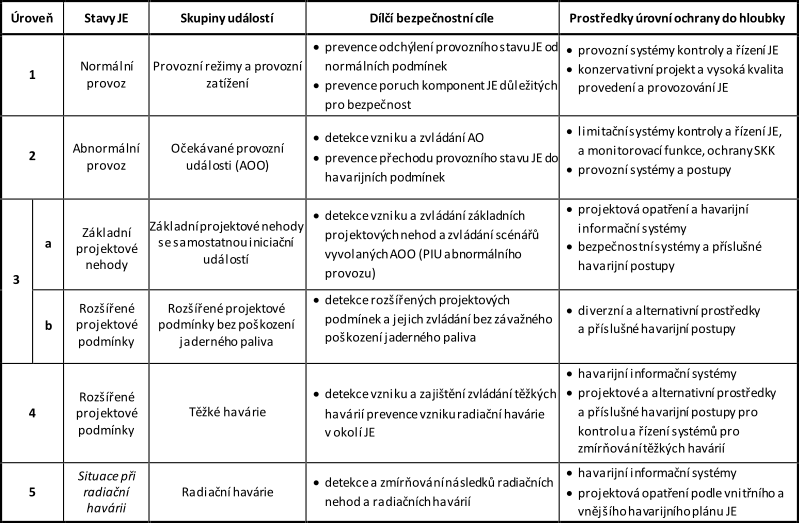
\includegraphics[width=\textwidth]{img/Úrovně ochrany do hloubky.png}
    \caption{Úrovně ochrany do hloubky.}
\end{figure}

\subsubsection{Fyzické bariéry DID}

Počet jednotlivých bariér závisí na zdrojovém členu (ETE jich má 5), účinnosti bariér, pravděpodobnosti výskytu a závažnosti nepříznivých interních i externích událostí.

Projekt musí zabránit ohrožení integrity fyzických bariér, a to zejména poslední a tím zabránit úniku RA látek do ŽP. Cílem je však zamezení selhání jedné nebo více bariér při ohrožení.

Vyloučit závislost, tj. zabránit selhání jedné bariéry v důsledku selhání jiné bariéry (stejné jako pro jednotlivé úrovně DID).

Není dovolen provoz při selhání jedné z bariér (jedná se o výzmnou událost a je nutné prošetřit).

\begin{enumerate}
	\item Palivová tableta -- chemická a fyzikální struktura paliva.
	\item Pokrytí palivových proutků -- hermetická hranice.
	\item Tlaková hranice primárního okruhu.
	\item Kontejnment (nebo jiný systém lokalizace RA látek pokud nemám kontejment $\rightarrow$ barbotážní věž).
\end{enumerate}

\begin{figure}[h!]
    \centering
    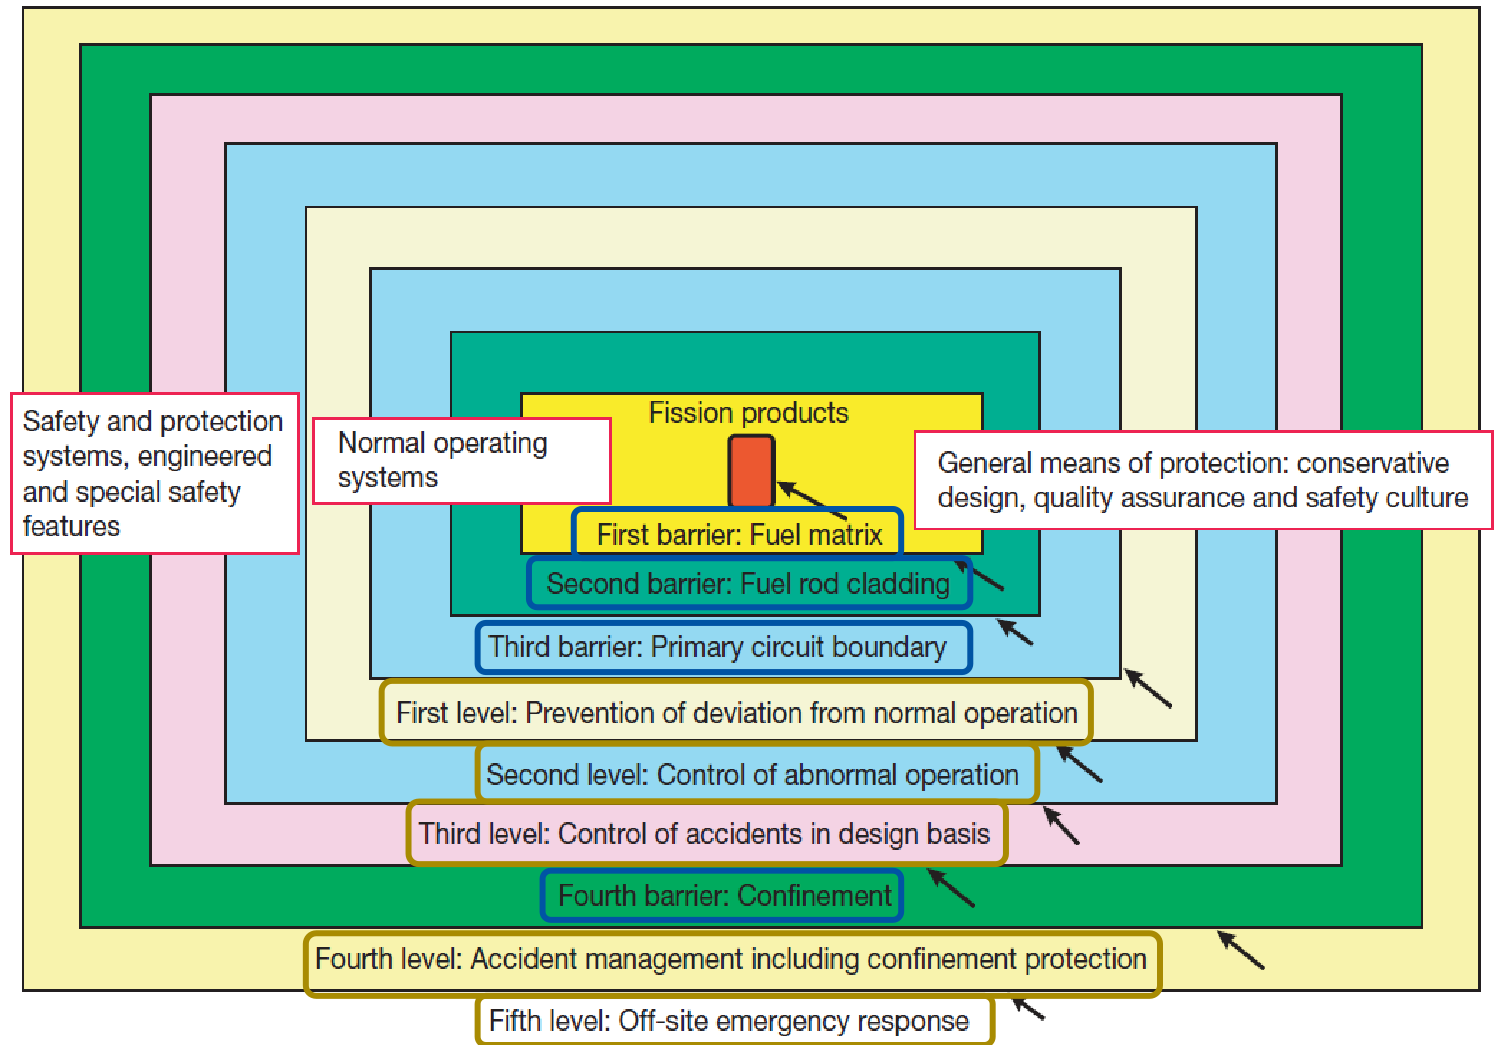
\includegraphics[width=\textwidth]{img/DiD-bariery.png}
    \caption{Bariéry a úrovně ochrany do hloubky.}
\end{figure}